\chapter{Implementation}\label{Implementation}

\section{ISA}

In this section we will briefly highlight the ISA of our DLX implementation.
This consists in: 
\begin{itemize}
    \item the control word and the meaning of each bit;
\end{itemize}
\begin{itemize}
    \item the implemented instructions and their behavior;
\end{itemize}
\begin{itemize}
    \item the way dependencies must be handled in order for the CPU to work.
\end{itemize}

\subsection{Control word structure}

The control word, generated by the controller at each clock cycle, is made of 33 bits. 
Here is its description: the different signals are grouped based on the stage in which they are used.

\begin{markdown}
- Decode stage

    - `rf_rd1, cw(32)`: enables the read port 1 of the register file.

    - `rf_rd2, cw(31)`: enables the read port 2 of the register file.

    - `se_signed_unsigned_bar, cw(30)`: when it is zero, the immediate is zero-extended to 32 bits (it's treated as an unsigned number), otherwise it's sign-extended.  

    - `se_size_16_26_bar, cw(29)`: when it is zero, the immediate is `IR[25:0]` and will be always zero-extended, otherwise it is `IR[15:0]` and `se_signed_unsigned_bar` will be taken into account.

- Execution Stage

    - `ex_sel_a, cw(28)`: when it is zero, the first operand of the execution stage is the NPC, otherwise it is the output of port 1 of the register file.

    - `ex_sel_b, cw(27)`: when it is zero, the second operand of the execution stage is the extended immediate value, otherwise it is the output of port 2 of the register file.

    - `alu_sub_add_bar, cw(26)`: when it is zero the adder performs an addition, otherwise a subtraction.

    - `alu_logic_sel, cw(25 downto 22)`: defines which logic operation to perform (and, or, xor, nor, etc.).

    - `alu_shift_sel, cw(21 downto 20)`: defines which shift operation to perform (logical left shift, arithmetic right shift, etc.).

    - `mul_start, cw(19)`: when it is one, a multiplication will start after one clock cycle.

    - `div_start, cw(18)`: when it is one, a division will start after one clock cycle.

    - `div_signed_unsigned_bar, cw(17)`: when it is zero, the division operands are treated as unsigned, otherwise they are treated as signed.

    - `div_sel, cw(16)`: when it is zero, the division's remainder will be selected, else the quotient will be returned.

    - `mul_sel, cw(15)`: when it is zero, the 32 LSBs of the product will be selected, else the 32 MSBs will be returned.

    - `cmp_config, cw(14 downto 12)`: defines which compare operation to perform (grater than, grater than or equal, etc.).

    - `ex_sel_out, cw(11 downto 9)`: is used to select which result of which component will be the output of the execution stage. 

    - `branch_eq_neq_bar, cw(8)`: when it is zero, the detector will check whether its input is equal to zero, else it will check if it is not equal to zero.

- Memory Stage

    - `mem_rw_wr_bar, cw(7)`: when it is zero, the memory is written to, else it is read from.

    - `mem_branch_enable, cw(6)`: when it is one a branch operation is being executed, so the PC is overwritten if the zero detector previously generated a one.

    - `mem_perform_jump, cw(5)`: when it is one a jump is being executed: the PC is always overwritten.

- Writeback Stage

    - `wb_sel, cw(4 downto 3)`: is used to select the contents of which register will be sent to the register file's write port.

    - `rf_sel_dest, cw(2)`: if zero, the destination address is read from `IR[20:16]`, else it's read from `IR[15:11]`.

    - `rf_write31, cw(1)`: if one, the write destination of the register file is automatically set to `r31` and the write address is ignored.

    - `rf_wr, cw(0)`: if one, enables the register file's write port.
 
\end{markdown}

\subsection{Instruction set}

The list of available instructions is in \autoref{tab:instructionset}.
With respect to the base version of the DLX, we added: nand, nandi, nor, nori, xnor, xnori, slt, slti, sgt, sgti, seq, seqi, smulh, smull, uquot, urem, squot, srem, ret.

We decided to avoid inserting the control words of each instruction in this table for brevity; nonetheless, the complete list of control words can be found in the spreadsheet inside the \texttt{doc} folder of the project.

\begin{table}[]
    \centering
    \begin{tabular}{|c|c|c|c|}
        \hline
         Mnemonic & Opcode & Example & Operation \\
         \hline

add & \texttt{0x00} & \texttt{add rx, ry, rz} & \texttt{RF[x] = RF[y] + RF[z]} \\

addi & \texttt{0x01} & \texttt{add rx, ry, imm\_16} & \texttt{RF[x] = RF[y] + imm\_16} \\

and & \texttt{0x02} & \texttt{and rx, ry, rz} & \texttt{RF[x] = RF[y] \& RF[z]} \\

andi & \texttt{0x03} & \texttt{andi rx, ry, imm\_16} & \texttt{RF[x] = RF[y] \& imm\_16} \\

nor & \texttt{0x04} & \texttt{nor rx, ry, rz} & \texttt{RF[x] = !(RF[y] | RF[z])} \\

nori & \texttt{0x05} & \texttt{nori rx, ry, imm\_16} & \texttt{RF[x] = not(RF[y] | imm\_16)} \\

nand  & \texttt{0x06} & \texttt{nand rx, ry, rz} & \texttt{RF[x] = !(RF[y] \& RF[z])} \\

nandi & \texttt{0x07} & \texttt{nandi rx, ry, imm\_16} & \texttt{RF[x] = not(RF[y] \& imm\_16)} \\

xnor & \texttt{0x08} & \texttt{xnor rx, ry, rz} & \texttt{RF[x] = !(RF[y] \^ RF[z])} \\

xnori & \texttt{0x09} & \texttt{xnori rx, ry, imm\_16} & \texttt{RF[x] = not(RF[y] \^ imm\_16)} \\

beqz & \texttt{0x0a} & \texttt{beqz rx, imm\_16} & \texttt{PC = (RF[x]) ? PC + 4 : (PC + 4 + imm\_16)} \\

bnez & \texttt{0x0b} & \texttt{bnez rx, imm\_16} & \texttt{PC = (RF[x]) ? (PC + 4 + imm\_16) : PC + 4} \\

j & \texttt{0x0c} & \texttt{j imm\_26} & \texttt{PC = PC + 4 + imm\_26} \\

jal & \texttt{0x0d} & \texttt{jal imm\_26} &\texttt{PC = PC + 4 + imm\_26; RF[31] = PC + 4} \\

lw & \texttt{0x0e} & \texttt{lw ry, imm\_16(rx)} &\texttt{ry = MEM[rx + imm\_16]} \\

nop & \texttt{0x0f} & \texttt{nop} & Nothing \\

or & \texttt{0x10} & \texttt{or rx, ry, rz} & \texttt{RF[x] = RF[y] | RF[z]} \\

ori & \texttt{0x11} & \texttt{ori rx, ry, imm\_16} & \texttt{RF[x] = RF[y] | imm\_16} \\

sge & \texttt{0x12} & \texttt{sge rx, ry, rz} & \texttt{rx = (ry >= rz) ? 1 : 0} \\

sgei & \texttt{0x13} & \texttt{sgei rx, ry, imm\_16} & \texttt{rx = (ry >= imm\_16) ? 1 : 0} \\

sle & \texttt{0x14} & \texttt{sle rx, ry, rz} & \texttt{rx = (ry <= rz) ? 1 : 0} \\

slei & \texttt{0x15} & \texttt{slei rx, ry, imm\_16} & \texttt{rx = (ry <= imm\_16) ? 1 : 0} \\

sne & \texttt{0x16} & \texttt{sne rx, ry, rz} & \texttt{rx = (ry != rz) ? 1 : 0} \\

snei & \texttt{0x17} & \texttt{snei rx, ry, imm\_16} & \texttt{rx = (ry != imm\_16) ? 1 : 0} \\

seq & \texttt{0x18} & \texttt{seq rx, ry, rz} & \texttt{rx = (ry == rz) ? 1 : 0} \\

seqi & \texttt{0x19} & \texttt{seqi rx, ry, imm\_16} & \texttt{rx = (ry == imm\_16) ? 1 : 0} \\

slt & \texttt{0x1a} & \texttt{slt rx, ry, rz} & \texttt{rx = (ry < rz) ? 1 : 0} \\

slt & \texttt{0x1b} & \texttt{slti rx, ry, imm\_16} & \texttt{rx = (ry < imm\_16) ? 1 : 0} \\

sgt & \texttt{0x1c} & \texttt{sgt rx, ry, rz} & \texttt{rx = (ry > rz) ? 1 : 0} \\

sgti & \texttt{0x1d} & \texttt{sgti rx, ry, imm\_16} & \texttt{rx = (ry > imm\_16) ? 1 : 0} \\

sll & \texttt{0x1e} & \texttt{sll rx, ry, rz} & \texttt{rx = (ry << rz[4:0])} \\

slli & \texttt{0x1f} & \texttt{slli rx, ry, imm\_16} & \texttt{rx = (ry << imm\_16[4:0])} \\

srl & \texttt{0x20} & \texttt{srl rx, ry, rz} & \texttt{rx = (ry >> rz[4:0])} \\

srli & \texttt{0x21} & \texttt{srli rx, ry, imm\_16} & \texttt{rx = (ry >> imm\_16[4:0])} \\

sub  & \texttt{0x22} & \texttt{sub rx, ry, rz} & \texttt{RF[x] = RF[y] - RF[z]} \\

subi & \texttt{0x23} & \texttt{subi rx, ry, imm\_16} & \texttt{RF[x] = RF[y] - imm\_16} \\

sw  & \texttt{0x24} & \texttt{sw imm\_16(rx), ry} & \texttt{MEM[rx + imm\_16] = ry} \\

xor & \texttt{0x25} & \texttt{xor rx, ry, rz} & \texttt{RF[x] = RF[y] \^ RF[z]} \\

xori & \texttt{0x26} & \texttt{xori rx, ry, imm\_16} & \texttt{RF[x] = RF[y] \^ imm\_16} \\

smulh & \texttt{0x27} & \texttt{smulh rx, ry, rz} & \texttt{RF[x] = (RF[x]*RF[y])[63:32]} \\

smull & \texttt{0x28} & \texttt{smull rx, ry, rz} & \texttt{RF[x] = (RF[x]*RF[y])[31:0]} \\

uquot & \texttt{0x29} & \texttt{uquot rx, ry, rz} & \texttt{RF[z] = RF[y] // RF[z]} \\

urem & \texttt{0x2a} & \texttt{urem rx, ry, rz} & \texttt{RF[z] = RF[y] \% RF[z]} \\

squot & \texttt{0x2b} & \texttt{squot rx, ry, rz} & \texttt{RF[z] = RF[y] // RF[z]} \\

srem & \texttt{0x2c} & \texttt{srem rx, ry, rz} & \texttt{RF[z] = RF[y] \% RF[z]} \\

ret & \texttt{0x2d} & \texttt{ret rx} & \texttt{PC = RF[x]} \\
         \hline 
    \end{tabular}
    \caption{Instruction set of our DLX}
    \label{tab:instructionset}
\end{table}

\subsection{Dealing with dependencies}\label{dependencies}
\begin{markdown}    
Here are some highlights on how to handle dependencies in the code.
These rules must be followed in order for the CPU to work as expected.

- If a RAW hazard happens, there must be two instructions between the one which writes and the one which reads. In case this does not already happen in the code, some `nop` instructions are necessary.

- For instructions which modify the program counter, the number of required `nop` instructions is three, since the program counter is written during the *memory* stage.

- Two multi-cycle instructions must be separated by other two instructions. `nop` instructions are required if this is not the case in the program. The reason behind this is that the controller can only handle multi-cycle instruction at a time and will only consider the most recently fetched one.
\end{markdown}

\section{Components Overview}\label{components_overview}

To obtain a full working DLX processor we developed and used different components. They are:
\begin{itemize}
    \item IRAM;
\end{itemize}
    \begin{itemize}
        \item DRAM;
        \item Controller (implementation explained in \autoref{controller_ch});
        \item Zero detector;
        \item Comparator;
        \item Pipeline register (single- and multi-bit);
        \item Register file;
        \item Sign extender;
        \item Logic unit;
        \item Shifter;
        \item P4 Adder;
        \item Booth multiplier (implementation explained in \autoref{Chpater_Impl_mul});
        \item SRT Radix-4 divider (implementation explained in \autoref{Chapter_Impl_Div});
    \end{itemize}

 \subsection{IRAM}
 
The IRAM is the static, read-only instruction memory used from which the instructions to be executed are fetched. 
Its content is initialised by a process which reads from the \texttt{sim/IRAM\_init\_file.mem} file when reset signal is active.
During nominal operation it sends out its data on the \texttt{mem\_instr\_out} signal: the datapath receives the full instruction while the controller only receives the opcode (located in the 6 MSBs of the instructions). 


 \subsection{DRAM}

The DRAM is the data memory of the processor.
It is characterised by two different processes: one that is in charge of asynchronously reading, while the other is in charge of synchronously writing it on the positive edge of the clock or resetting it.
The signal \texttt{rw\_bar} discriminates between a read (the signal is one) and a write (the signal is zero) operation.

 
 \subsection{Zero detector}

The zero detector is used to compute whether a branch should be taken or not. 
Since there are the \texttt{beqz} and \texttt{bnez} instructions, we use the signal \texttt{branch\_eq\_neq\_bar} to discriminate between the two:
\begin{itemize}
    \item \texttt{branch\_eq\_neq\_bar} is zero: \texttt{bnez} instruction, so the output is one if the data input is not zero;
    \item \texttt{branch\_eq\_neq\_bar} is one: \texttt{beqz} instruction, so output is one if the data input is zero;

\end{itemize}

 
 \subsection{Comparator}

Exploiting the already implemented adder/subtractor, we added some logic to obtain a comparator. 
It takes as inputs the calculated difference and carry out of the adder and analyses the relation between the two operands $A$ and $B$, depending on \texttt{config} input (which is responsible of differentiating between the possible types of comparison). 
In particular:
\begin{itemize}
    \item \texttt{config} is \texttt{000}:  less than equal comparison, returns one if $A \leq B$;
    \item \texttt{config} is \texttt{001}: less than comparison, returns one if $A<B$;
    \item \texttt{config} is \texttt{010}: greater than comparison, returns one if $A>B$;
    \item \texttt{config} is \texttt{011}: greater than equal comparison, returns one if $A \geq B$;
    \item \texttt{config} is \texttt{100}: equal comparison, returns one if $A=B$;
    \item \texttt{config} is \texttt{101}: not equal comparison, returns one if $A\neq B$.
\end{itemize}

The result of the comparison is then zero-extended to 32 bits as it is handled like any other data by the datapath.

\subsection{Pipeline register}

This component is a simple Parallel-In-Parallel-Out N-bit or 1-bit register with an enable signal which is driven by the controller directly and is used to stall the pipeline in case of multi cycle operations.
These registers have been implemented as standalone components for the sake of cleaner, more reusable code.

\subsection{Register file}

The implemented register file is composed by 32 registers which are N bits wide, with two reading ports and one writing port. 
The enable signals are:
\begin{itemize}
    \item \texttt{RD1}: enables reading from reading port 1;
    \item \texttt{RD2}: enables reading from reading port 2;
    \item \texttt{WR}: enables writing;
    \item  \texttt{Write31}: when it is one the write destination of the register file is automatically set to r31 and the write address is ignored (it's used used by \texttt{jal} instructions).
\end{itemize}
Reading is asynchronous, while writing is synchronous on the falling edge of the clock to decrease the latency, as explained previously.

\subsection{Sign extender}

Sign-extension or zero-extension has to be performed both for I-type and J-type instructions, depending on the specific operation to be performed. 
To control the behaviour of the module two control signals have been defined:
\begin{itemize}
    \item \texttt{size\_16\_26\_bar}: when it is at one  the immediate is considered on 16 bits, otherwise is on 26 bits;
    \item \texttt{signed\_unsigned\_bar}: when it is one the immediate is sign-extended, otherwise is zero-extended.
\end{itemize}
In the case of 26-bit immediate (J-type instructions), this is always extended as signed.

\subsection{Logic unit}

The implemented logic unit is based on the T2 logic unit, in which there is a selection signal \texttt{S} on 4 bits that chooses one among different logic operations. 
This logic unit only computes the following function:
\[
Output = S_3 \cdot A \cdot B + S_2 \cdot A \cdot \overline{B} + S_1 \cdot \overline{A} \cdot B + S_0 \cdot \overline{A} \cdot \overline{B} 
\]
The values of \texttt{S} associated with each logic function are summarised in \autoref{tab:logic_func}.

\begin{table}[]
    \centering
    \begin{tabular}{|c|c|c|c|c|}
        \hline
         Function & $S_3$ & $S_2$ & $S_1$ & $S_0$\\
         \hline
          and & 1 & 0 & 0 & 0 \\
         nand & 0 & 1 & 1  & 1\\
         or & 1 & 1 & 1 & 0\\
         nor & 0 & 0 & 0  & 1\\
         xor & 0 & 1 & 1 & 0 \\
         xnor & 1 & 0 & 0 & 1 \\
         \hline 
    \end{tabular}
    \caption{Functions computed by the logic unit based on the value of \texttt{S}}
    \label{tab:logic_func}
\end{table}

\subsection{Shifter}

The unit implements the T2 barrel shifter on N bits, where N is a power of 2. 
It takes as inputs the value to shift, the amount of positions to shift it by (so only the six LSBs of the second operand are considered) and a 2-bit configuration signal to choose between logic/arithmetic and left/right shifts. 
The shift is performed by three successive operations: first a set of eight 71-bit masks is generated, then one of these masks is chosen, then only a 64-bit subsection of these masks is selected as the final output.

\subsection{P4 adder}

The adder shares the architecture of the one used in the Pentium 4 processor: using a sparse tree carry generator, only one of them is generated each four bits.
The carries are used by eight carry-select adders, in charge of computing 4 bits of the sum each.

The adder produces the result in one clock cycle. 
In particular, it can be used either as an adder or as a subtractor, depending on the value of  the \texttt{ALU\_SUB\_ADD\_BAR} signal. 
This signal, although it's conceptually used for control from an external point of view, internally it's used as a data signal. 
Due to the way two's complement works: 
\[
    \rvert A - B \rvert_2 = \rvert A + \overline{B} + 1 \rvert_2
\]

For this reason, the signal \texttt{ALU\_SUB\_ADD\_BAR} is used as carry-in and also to select the second operand between $B$ and $\overline{B}$.

\section{Simulation} \label{sim_chap}

In this section we will talk about the way you can simulate the processor, using the scripts we have written.

The simulation consists in providing the CPU some stimuli (i.e. an assembly program) and observing how the system reacts to them. 
In particular, it might be interesting to look at the internal signals, in order to understand whether the components and the pipeline are working correctly, and to see the state of the register file and of the memory at the end of the simulation.

The simulation is performed using the ModelSim simulation software; the scripts we provide have been tested on version 20.1 and 20.4.

In order to simulate, you need an assembly program.
This should be created inside the \texttt{sim/asm\_example} folder, using the same name both for the folder and for the \texttt{.asm} file.

The simulation can be run by executing \texttt{scripts/simulate.py}. 
You can pass many arguments to this script or none at all, in order to make the execution more flexible. 
It is in charge of calling other scripts and commands: at the end of each of them, it is possible to see the outcome of the process on the terminal. 
In particular, green text stands for success, while red stands for failure. 

Here is a brief explanation of each argument of the script:
\begin{itemize}
\item \texttt{-c, --compile\_only}: compile the VHDL files without executing them;
\item \texttt{-a ASM, --asm ASM}: which assembler file to execute;
\item \texttt{-g, --gui}: open ModelSim's GUI to analyse the produced waveforms;
\item \texttt{-p, --pretty}: prettify memory and register file dump;
\item \texttt{-v [KEY=VALUE \dots], --verify [KEY=VALUE \dots]}: define a list of key-expected\_value elements to be checked against the register file/dram dump's contents, executed only if \texttt{-p} is present.
\end{itemize}

With the flag \texttt{-c} the script just compiles the DLX. 
The list of files to be compiled is located in the \texttt{sim} folder. 
This can be useful in order to know if the code written does not contain any syntax errors.

With the command \texttt{-asm [FILE]} you can assemble a \texttt{.asm} file and use it to simulate the processor. 
The script stops in case the assembler produces some errors.

By default, the simulation does not open the gui of modelsim. 
All the commands needed for that are provided by \texttt{sim/simulation\_cli.do}.
Basically the simulation is run for 1 \si{\micro\second}, then it dumps the contents of register file and dram into the file \texttt{sim/dump\_rf\_dmem.dump}.
As a side note, it is highly suggested to add an endless loop at the end of you program to avoid unexpected behaviours after its execution is completed.

The content of the dump file as-is is not very readable, since it is only the list of all the values inside the two components.
Using the flag \texttt{-p}, another script is run which prettifies the dump.
\autoref{fig:dump_file} shows an example of the register file part of a dump after it has been prettified.

The last option of the script is the auto-verification of the values stored in the register file and/or dram. 
Using the \texttt{-v} option, you can provide a list of key-value pairs which are expected to be in the dump. 
Each element of this list is separated by the others using a space.
A key can either be a register (using the structure \texttt{rX}, with \texttt{X} between 0 and 31) or a memory location (using the structure \texttt{mX}, with \texttt{X} between 0 and 255).
The expected value can be written both in hexadecimal (in the form \texttt{0xXXXXXXXX}, has to be exactly 8 digits long) or as an unsigned decimal.

Let's say that you want to check whether, at the end of the simulation, the register 1 has value \texttt{0x001abde7} while the dram cell 0 has value 3628800. 
To do so, you would execute \texttt{scripts/simulate.py -a your\_file.asm -p -v r1=0x001abde7 m0=3628800}.

\begin{figure}
    \centering
    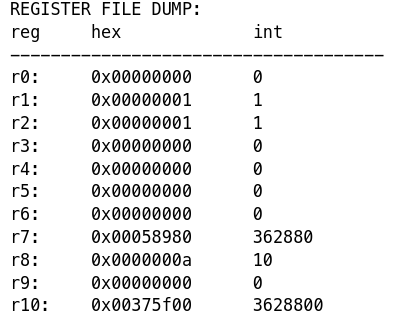
\includegraphics[width=70mm]{images/dump_ex.png}
    \caption{Example of dump file (only the first few lines)}
    \label{fig:dump_file}
\end{figure}

At the end of the execution, the script will show you whether the checks were successful or not. 
In \autoref{fig:result_simulation} you can find an example of the output should a check fail.

\begin{figure}
    \centering
    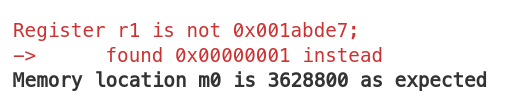
\includegraphics[width=70mm]{images/result_simulation.png}
    \caption{Result of a simulation using the \texttt{-v} flag}
    \label{fig:result_simulation}
\end{figure}

If you also want to have a look at the generated waveforms, in addition to all of the CLI options provided so far, you can add the \texttt{-gui} option when executing the script. 
After successful compilation, ModelSim will open and the system will ready to be run, using the \texttt{run time X} command in software's terminal. 

The script automatically adds to the waveform viewer all the important signals of the CPU (basically everything related to the pipeline); the signals are grouped by stage.
Different colours are used as well, one per stage, in order to improve readability.

\section{Synthesis} \label{syn_chap}

The synthesis process has been done using Synopys Design Compiler.
The process has been done in a simple way, without considering other possible optimisations. 

The first step is to analyze the files, in order to see whether they can be synthesised or not. 
The first time we did so, we discovered that most of our DLX was fine except for the register file: the writing operation happens on the negative edge of the clock, but the technology library we employed does not have a negative-edge triggered flip flop, so there was no way to synthesise it. 
In order to keep the component's behaviour unchanged, the clock inside the register file is inverted and its rising edge is used to perform a write operation.

The synthesis script located in \texttt{syn/syn\_script.tcl} shows all the commands we used to perform the synthesis. 

We decided not to spend much time at this stage (for instance, we could have uses the switching activity of the system to improve the power analysis, or to adopt the clock gating technique to decrease power consumption). 

The final reports show a very slow critical path, around 6.5 \si{\nano\second}, which is the carry propagation through the ripple carry adder used inside the multiplier. 
Because of this, the synthesis has been performed with a global timing constraint of 7 \si{\nano\second}, which means that our DLX would run at $\sim 142.8$ \si{\MHz}.
A possible optimisation may consists of using a 64-bit P4 adder inside the multiplier, in order to improve the critical path. 
Another possibility would be to replace the 64-bit multiplier with a 32-bit one: this would reduce the functionalities of the CPU, but improve the delay.
Another possible optimisation would be to pipeline the multiplier by splitting the 64-bit sum in two subsequent 32-bit sums that would happen in two different clock cycles (this would double the latency of the multiplication). 

The results about the estimated power consumption are shown in \autoref{tab:power_consumption}. 
The overall area occupation is 19616 \si{\micro\meter\squared}.

\begin{table}[]
    \centering
    \begin{tabular}{|c|c|c|c|c|}
\hline
Power Group & Internal Power & Switching Power & Leakage Power & Total Power\\
\hline
    IO pad & 0 & 0  & 0 &  0 \\
    Memory & 0 & 0  & 0 &  0 \\
    Black Box & 0 & 0 & 0 &  0 \\
    Clock Network & $172.7068$ & $1.7301\cdot10^5$ & $28.7064$ & $1.7318\cdot 10^5$ \\
    Register & 1.7912$\cdot 10^3$ & 8.1986 & 1.4242$\cdot 10^5$ & 1.9418$\cdot 10^3$ \\
    Sequential & 1.7210$\cdot 10^{-2}$ & 7.2383$\cdot 10^{-4}$ & 3.9772$\cdot 10^3$ & 3.9952 \\
    Combinational & 44.4411 & 115.3323 & 2.4928$\cdot 10^5$ & 409.0535 \\
\hline
Total & $2.0083 \cdot 10^3$ & $1.7313 \cdot 10^5$ & $3.9570 \cdot 10^5$ & $1.7554 \cdot 10^5$ \\
\hline
    \end{tabular}
    \caption{Post synthesis power consumption in \si{\micro\watt}}
    \label{tab:power_consumption}
\end{table}

\section{Physical Design}

The placing and routing of the DLX processor has been done through the aid of Cadence Innovus Implementation System.

First we created the configuration files for Innovus, such as the \texttt{.globals} and \texttt{.view} files, so that they pointed to the post-synthesis netlist and SDC files. 
Then we proceeded to the structuring of the floorplan, defining the aspect ratio of the die and inserting the power rings using high metal layers to avoid congestion (M9 for horizontal lines and M10 for vertical lines). 

In order to distribute the power and ground signals across the chip to the cells, vertical and horizontal metal wires were added and routed.
The metal layers 1 to 8 were allocated to the cells, avoiding the higher levels which are reserved to for the power grid.

As it was requested to place the memories outside the processor, we needed to place their connection pins along the left and right edges of the chip. 
Along with these pins we also added the clock and reset ones at the top of the die .

For structural reasons we completed the placement by inserting filler cells in the free spaces, in order not to leave any empty space. 
Finally we performed the signal routing.

Analyses for timing have been done in order to understand if any violation might have occurred and we verified that we obtained positive slack both for setup and hold times.

The reports generated state that our DLX occupies a total area of 18798.5 \si{\micro\meter\squared}, is made of 23557 gates and 10486 cells.

In \autoref{fig:amoeba_view}  and \ref{fig:phy-view} we can see the amoeba view and the physical view of our processor.
It is interesting to notice that the datapath occupies almost the entire die area, while the area occupation of the controller (whose components are the white rectangles in the top-right quarter of the amoeba view) is minimal. 
\begin{figure}
    \centering
    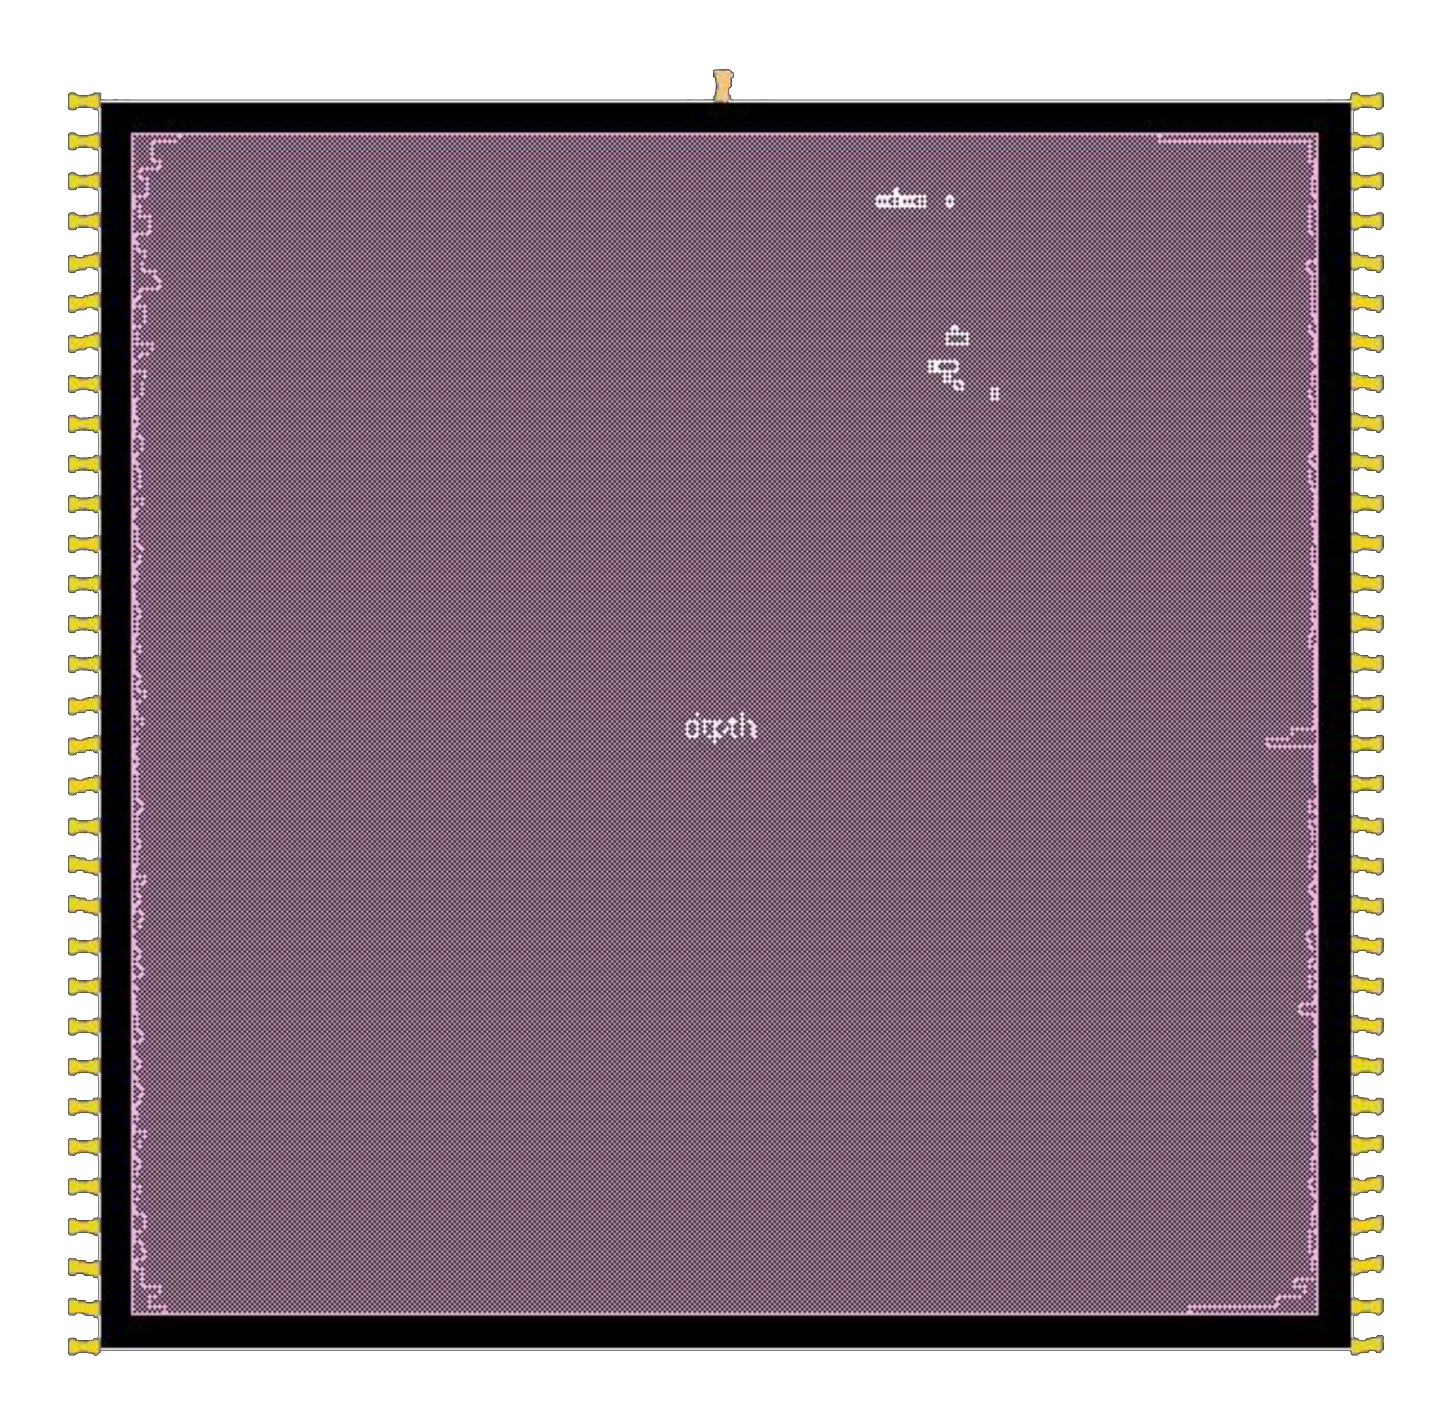
\includegraphics[width=0.7\linewidth]{images/amoeba_view.png}
    \caption{Amoeba view of the DLX}
    \label{fig:amoeba_view}
\end{figure}
\begin{figure}
    \centering
    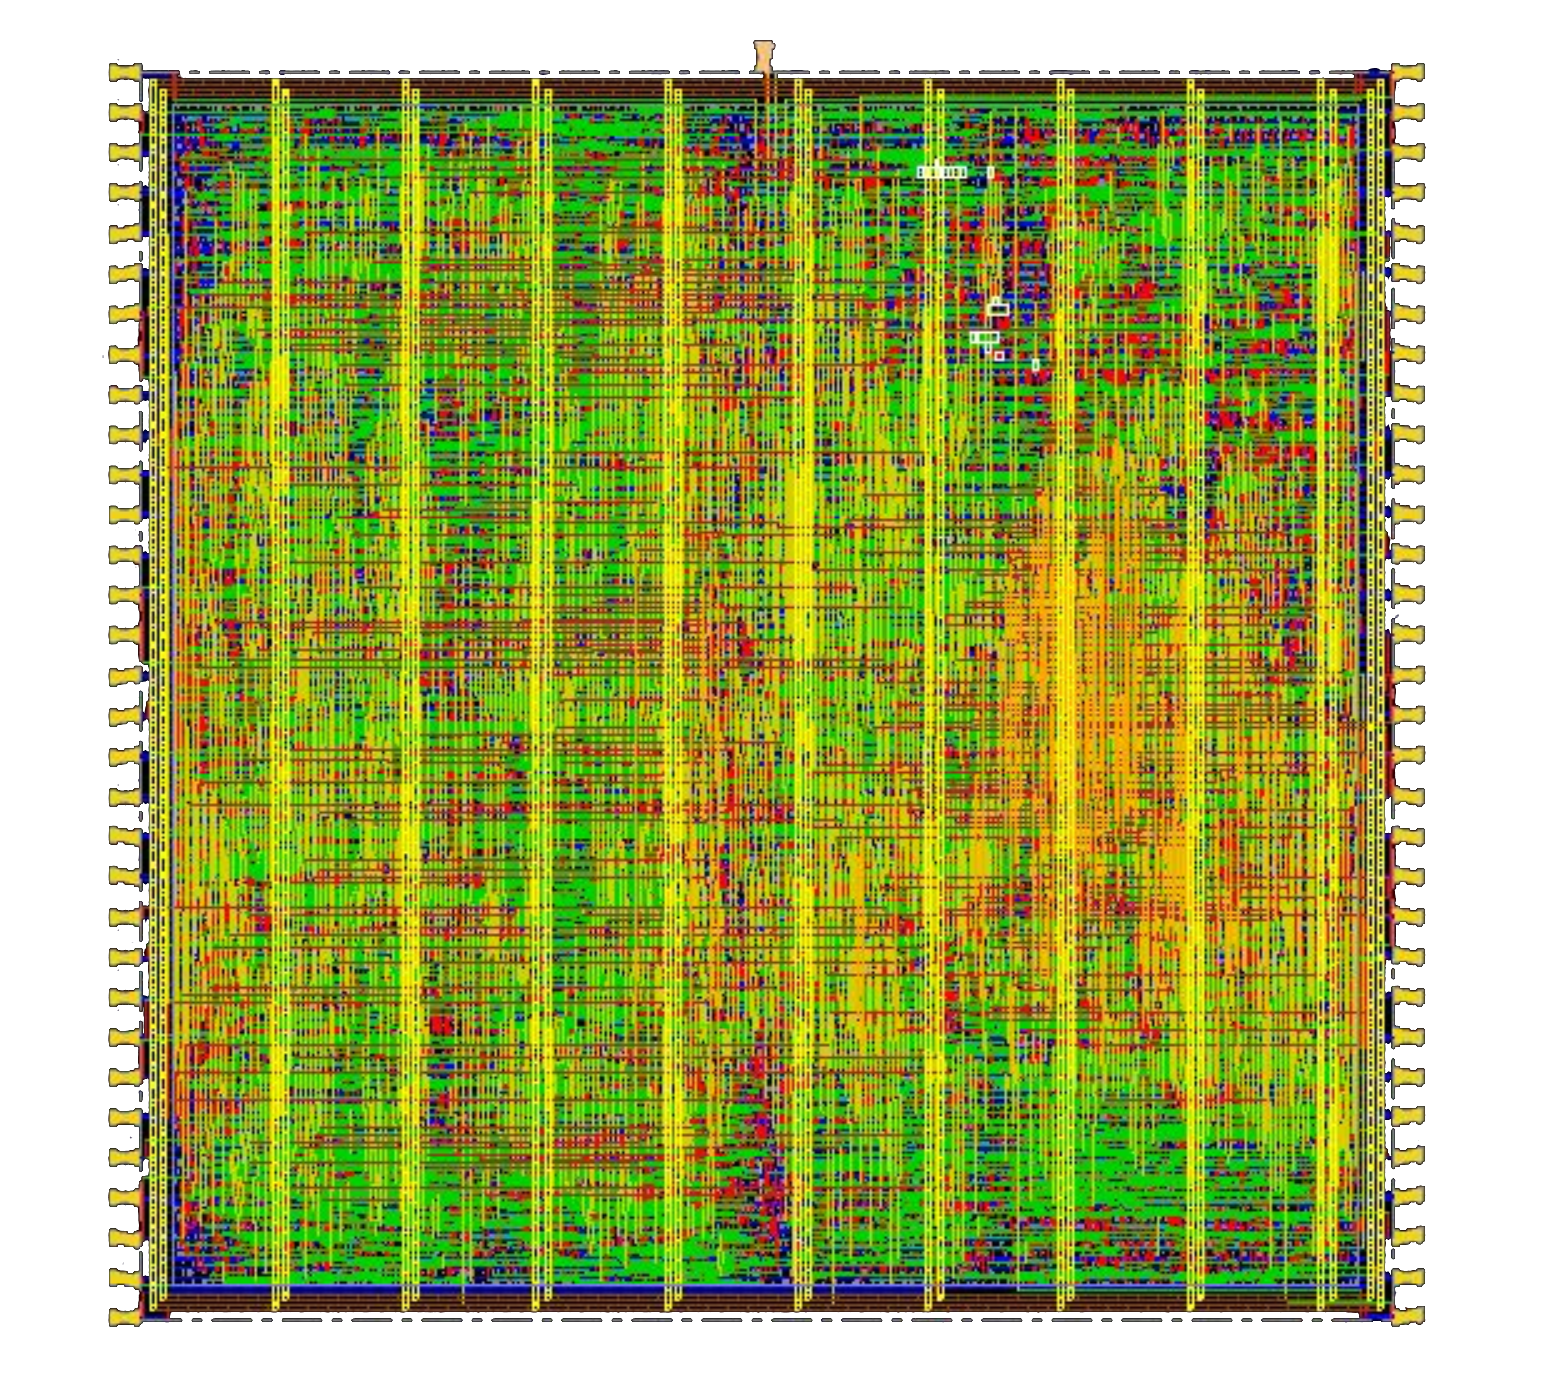
\includegraphics[width=0.7\linewidth]{images/phy_view.png}
    \caption{Physical view of the DLX}
    \label{fig:phy-view}
\end{figure}